\documentclass{article}
\usepackage{graphicx}
\usepackage{geometry}
\usepackage{hyperref}
\usepackage{booktabs}
\usepackage{subcaption}
\usepackage{amsmath}

\geometry{
    a4paper,
    margin=0.7in
}

\hypersetup{
    colorlinks=true,
    linkcolor=blue,
    filecolor=magenta,      
    urlcolor=cyan,
}

\title{SNN vs CNN Baseline Robustness Comparison\\Sweep under Data Heterogeneity ($f \le 5$)}
\author{ByzFL SNN Benchmark}
\date{\today}

\begin{document}

\maketitle

\section{Introduction}
This document presents a detailed robustness comparison between a Spiking Neural Network (SNN) with surrogate gradient scaling $\alpha=1.0$ and a standard Artificial Neural Network (CNN) baseline. Both models are evaluated on the MNIST dataset under identical client partitioning and attack scenarios:
\begin{itemize}
    \item \textbf{Byzantine Nodes}: $f \in \{0, 1, 2, 3, 4, 5\}$ out of $N=10$ honest nodes
    \item \textbf{Data Heterogeneity}: Non-IID levels $\gamma \in \{1.0, 0.66, 0.33, 0.0\}$
    \item \textbf{Attack Model}: Optimal A Little Is Enough (\texttt{Optimal\_ALittleIsEnough\_neg1})
    \item \textbf{Aggregators}: Best aggregated result across Centered Clipping and Geometric Median (pre-aggregated with NNM and ARC).
\end{itemize}

\section{Visual Heatmaps Comparison}
The figure below places the aggregated test accuracy heatmaps of the SNN ($\alpha=1.0$) and the CNN baseline side-by-side.

\begin{figure}[htbp]
    \centering
    \begin{subfigure}[b]{0.48\textwidth}
        \centering
        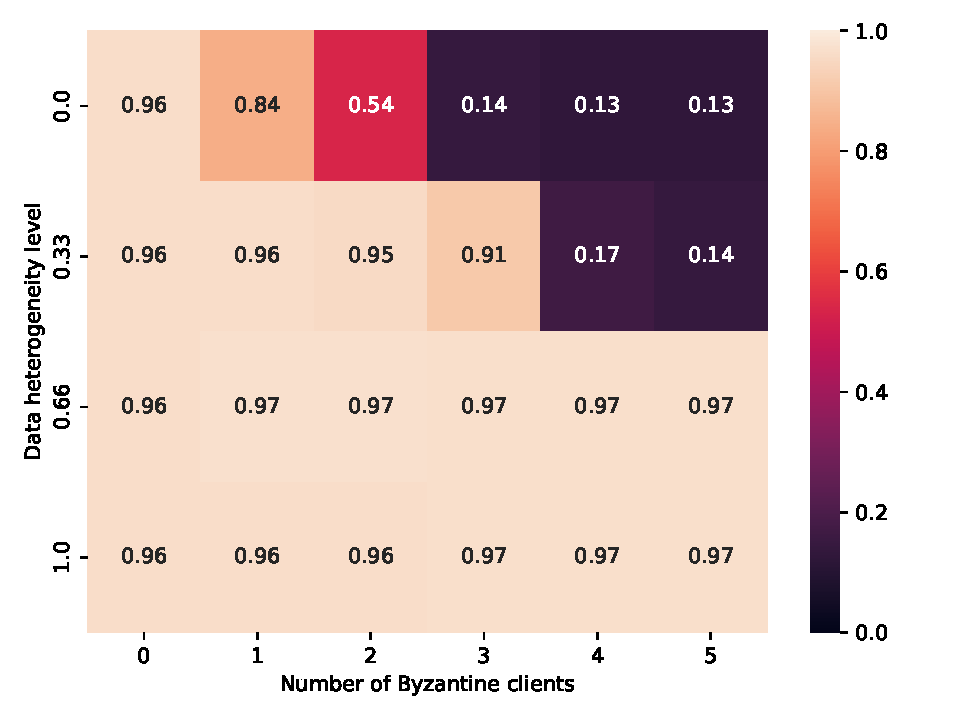
\includegraphics[width=\textwidth]{heatmap_snn_alpha_1_0.pdf}
        \caption{SNN ($\alpha = 1.0$)}
        \label{fig:heatmap_snn}
    \end{subfigure}
    \hfill
    \begin{subfigure}[b]{0.48\textwidth}
        \centering
        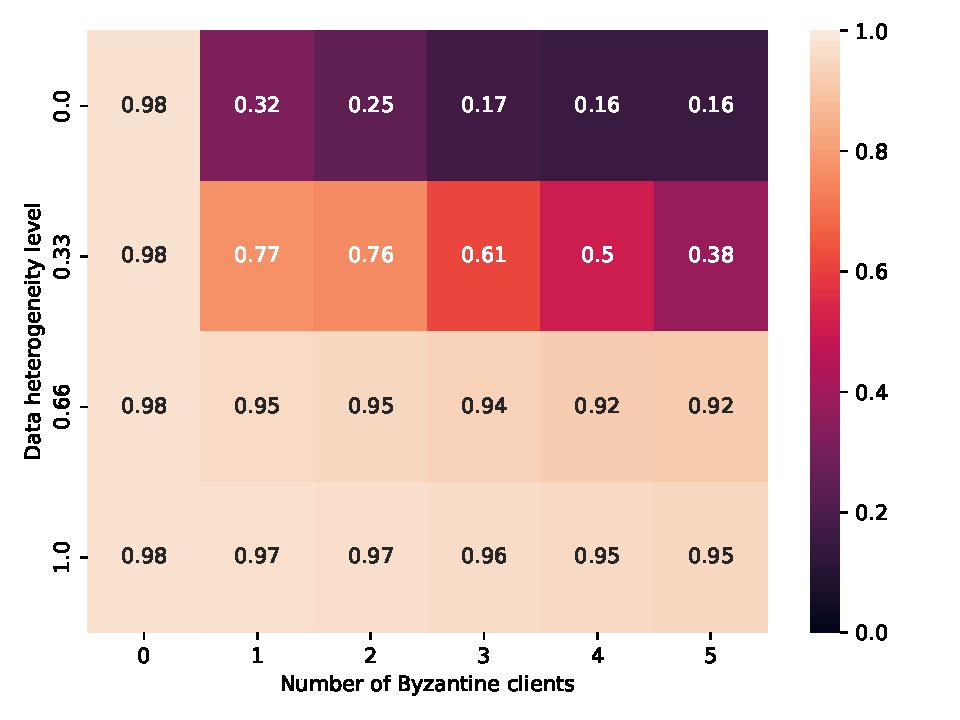
\includegraphics[width=\textwidth]{heatmap_cnn_baseline.pdf}
        \caption{CNN Baseline}
        \label{fig:heatmap_cnn}
    \end{subfigure}
    \caption{Aggregated Test Accuracy Heatmaps for SNN vs CNN baseline ($f \le 5$).}
    \label{fig:heatmaps_comparison}
\end{figure}

\newpage

\section{Quantitative Detailed Tables}

\subsection{SNN (ArcTangent, $\alpha = 1.0$, $T=10$)}
\begin{table}[htbp]
    \centering
    \begin{tabular}{ccccccc}
        \toprule
        & \textbf{f = 0} & \textbf{f = 1} & \textbf{f = 2} & \textbf{f = 3} & \textbf{f = 4} & \textbf{f = 5} \\
        \midrule
        $\gamma = 1.0$ & 96.43\% & 96.42\% & 96.48\% & 96.52\% & 96.60\% & 96.63\% \\
        $\gamma = 0.66$ & 96.43\% & 96.90\% & 96.98\% & 96.75\% & 96.66\% & 96.53\% \\
        $\gamma = 0.33$ & 96.46\% & 96.45\% & 95.44\% & 90.66\% & 16.66\% & 14.21\% \\
        $\gamma = 0.0$ & 96.41\% & 84.02\% & 53.80\% & 14.22\% & 12.63\% & 12.63\% \\
        \bottomrule
    \end{tabular}
    \caption{Aggregated test accuracy for SNN ($\alpha=1.0$).}
\end{table}

\subsection{CNN Baseline (NLLLoss, lr=0.05)}
\begin{table}[htbp]
    \centering
    \begin{tabular}{ccccccc}
        \toprule
        & \textbf{f = 0} & \textbf{f = 1} & \textbf{f = 2} & \textbf{f = 3} & \textbf{f = 4} & \textbf{f = 5} \\
        \midrule
        $\gamma = 1.0$ & 97.58\% & 97.51\% & 97.19\% & 97.18\% & 96.90\% & 96.70\% \\
        $\gamma = 0.66$ & 97.56\% & 96.92\% & 96.21\% & 96.08\% & 95.16\% & 95.07\% \\
        $\gamma = 0.33$ & 97.58\% & 86.33\% & 81.27\% & 82.89\% & 57.49\% & 52.26\% \\
        $\gamma = 0.0$ & 97.55\% & 55.41\% & 47.28\% & 17.42\% & 15.96\% & 15.96\% \\
        \bottomrule
    \end{tabular}
    \caption{Aggregated test accuracy for CNN baseline.}
\end{table}

\section{Key Insights}
\begin{itemize}
    \item \textbf{Low-Heterogeneity Regime ($\gamma \ge 0.66$)}: SNN ($\alpha=1.0$) shows superior resilience to large Byzantine fractions compared to CNN. At $\gamma=0.66$ and $f=5$, the SNN accuracy remains at \textbf{96.53\%} while the CNN drops to \textbf{95.07\%}.
    \item \textbf{High-Heterogeneity Regime ($\gamma = 0.0$)}: Under the extreme non-IID regime, the SNN shows significant gains in the low-to-moderate attacker counts:
    \begin{itemize}
        \item Under $f=1$, SNN achieves \textbf{84.02\%} accuracy compared to CNN's \textbf{55.41\%} (+28.6\% improvement).
        \item Under $f=2$, SNN achieves \textbf{53.80\%} accuracy compared to CNN's \textbf{47.28\%} (+6.5\% improvement).
    \end{itemize}
    \item \textbf{Attacker count breakdown threshold}: For larger numbers of attackers ($f \ge 4$), the CNN baseline remains stable for a longer period at $\gamma=0.33$ ($57.49\%$), whereas SNN collapses.
\end{itemize}

\end{document}
